\documentclass[11pt]{article}
\usepackage[utf8]{inputenc}
\usepackage{amsmath, amsfonts, amssymb}
\usepackage{graphicx}
\usepackage{geometry}
\usepackage{booktabs}
\usepackage{hyperref}
\usepackage{microtype}
\usepackage{xcolor} % TEMPORARY: marks Claude's additions in blue

\geometry{margin=1in}

\title{Homework Assignment 4: Studention Transport Monte Carlo Simulation}
\author{Tal Ramot}
\date{\today}

\begin{document}

\maketitle

\section*{Introduction}
This report details the results of an explicit Monte Carlo simulation of Studention transport in a sphere of Exercisium. Exercisium is a fissile material with atomic weight $A = 300$, density $\rho = 30$ g/cm$^3$, and a microscopic cross section $\Sigma_t = 10$ barn. 

The simulation advanced active Studentions generation-by-generation. For each Studention, the distance to the next event is determined by $s = -\ln(\xi) / \Sigma_{macro}$. If the advanced particle leaves the sphere radius $R$, it is deleted. Otherwise, the type of collision is determined probabilistically:
\begin{itemize}
    \item \textbf{Absorption} ($P_0 = 20\%$): The Studention disappears.
    \item \textbf{Scattering} ($P_1 = 50\%$): The Studention scatters in a random 3D direction.
    \item \textbf{Fission} ($P_2 = 30\%$): The original is absorbed, and two new Studentions are emitted in independent random directions.
\end{itemize}

A sphere is considered critical if at least one of 100 histories starting at the origin becomes critical (surpassing 10,000 active particles). Otherwise, the sphere is noncritical.

\section*{Question 1: Critical Radius of the Base Case}
Running the bisection search with $N = 100$ histories per check yielded:
\begin{itemize}
    \item \textbf{Critical Radius:} $8.5417 \pm 0.2084~\text{cm}$
    \item \textbf{Critical Mass:} $78.3136\pm  0.1907~\text{kg}$
\end{itemize}

\newpage
\section*{Question 2: Critical Mass vs. Density}
The simulation was executed for 11 densities linearly spaced between 10 g/cm$^3$ and 100 g/cm$^3$. The resulting critical radius and critical mass are plotted on a logarithmic scale in Figure~\ref{fig:density}.

\begin{figure}[hbt!]
    \centering
    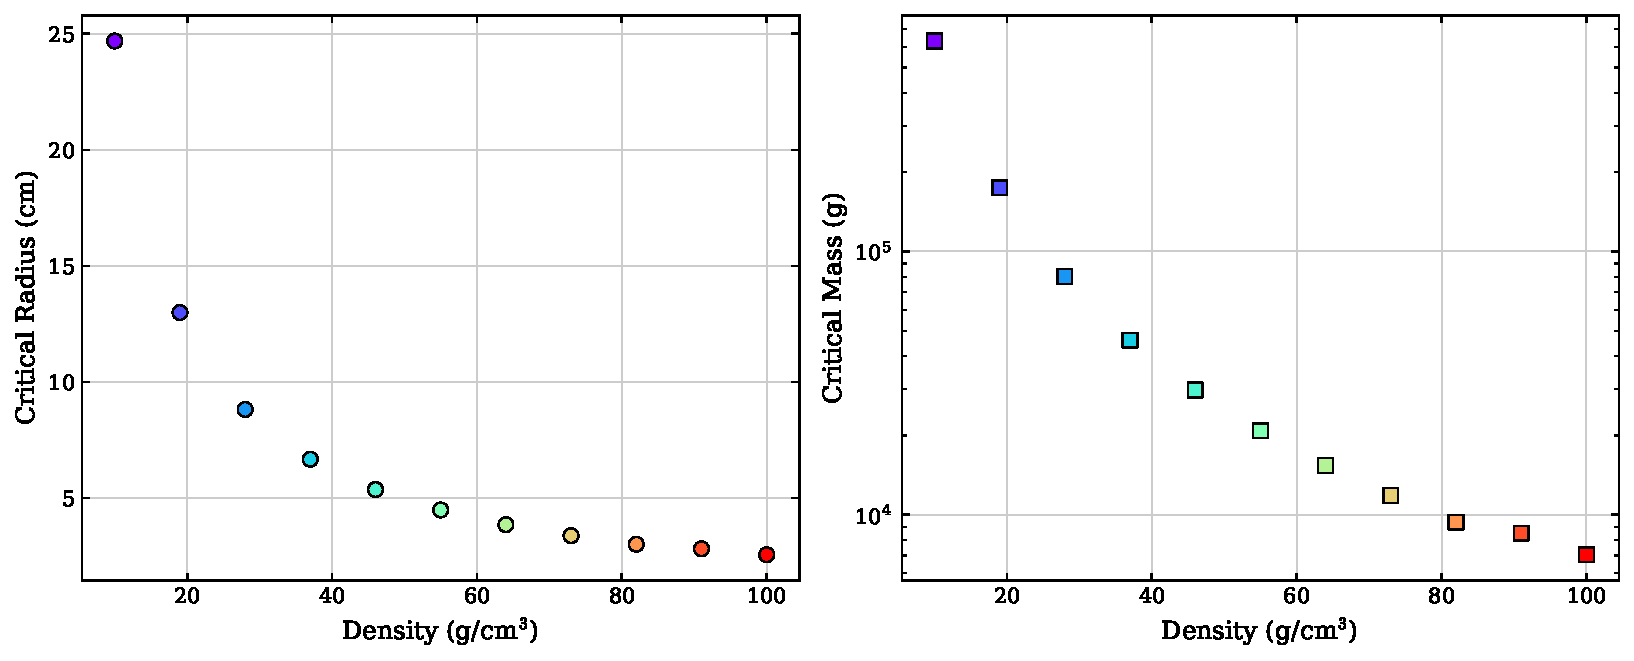
\includegraphics[width=0.75\textwidth]{figs/density_analysis.pdf}
    \caption{Critical radius (cm) and critical mass (g) as a function of Exercisium density.}
    \label{fig:density}
\end{figure}

\subsection*{Discussion}
As the density increases, the mfp (mean free path) decreases, making it less likely for Studentions to escape the sphere at a certain radius. This results in a smaller critical radius, and it is the cause of the decreasing fashion of the graphs in Figure~\ref{fig:density}. 

\newpage
\section*{Question 3: Probability Grid \& Parameterization}
The critical radius and critical mass were evaluated across 13 different collision probability configurations. The results are plotted against the multiplication parameter $c = P_1 + 2P_2$ in Figure~\ref{fig:probability}.

\begin{figure}[hbt!]
    \centering
    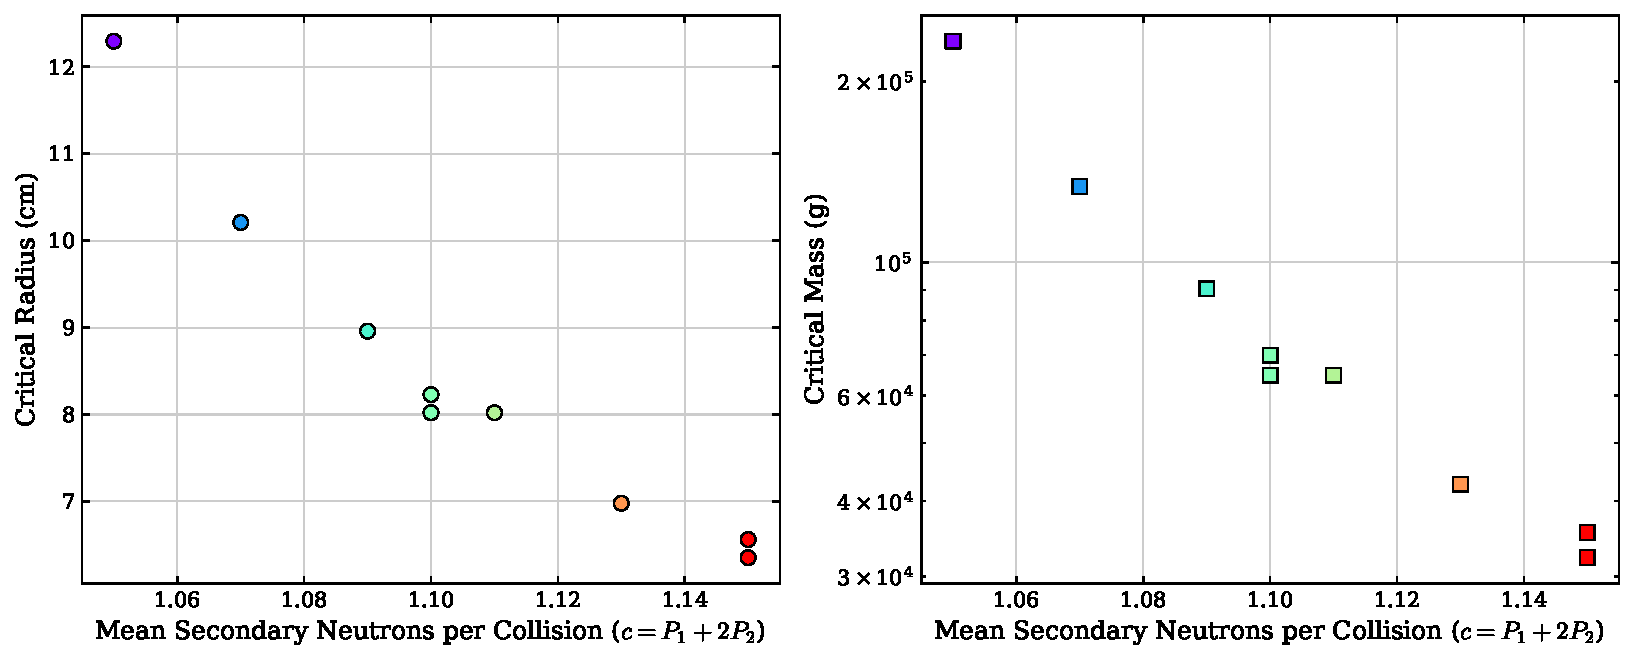
\includegraphics[width=0.75\textwidth]{figs/probability_analysis.pdf}
    \caption{Critical radius (cm) and critical mass (g) as a function of the multiplication parameter $c = P_1 + 2P_2$.}
    \label{fig:probability}
\end{figure}

\subsection*{Discussion}
In figure \ref{fig:probability}, we can notice that the critical mass is uniquely determined by the average secondary Studention count $c$ and is not affected by the separate values of $P_0, P_1$, and $P_2$. As explained in the previous discussion, the shorter the mfp is, the smaller the critical radius is - because the Studention is less likely to escape the sphere at a certain radius. In addition, the more secondary Studentions are produced, the more likely it is that at least one of them will not escape the sphere at a certain radius, so the critical radius is also smaller. This is the decreasing fashion of the graphs in Figure~\ref{fig:probability}. 

\newpage
\section*{Question 4: Deep Probability Sweep}
A wider grid of 33 different probability configurations was simulated to analyze the critical radius and mass across a broad range of $c$. The results are shown in Figure~\ref{fig:deep_probability}.

\begin{figure}[hbt!]
    \centering
    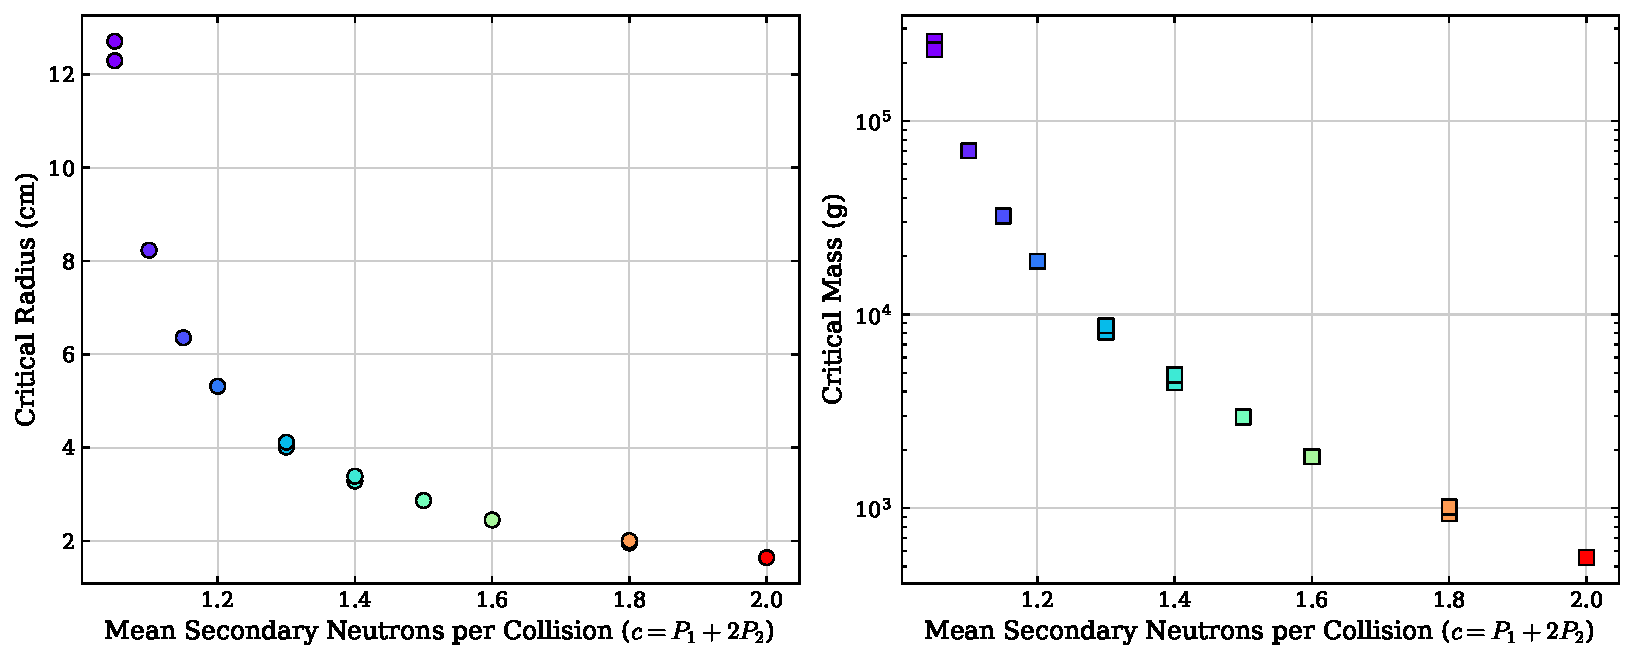
\includegraphics[width=0.75\textwidth]{figs/deep_probability_analysis.pdf}
    \caption{Critical radius (cm) and critical mass (g) for 33 configurations as a function of the multiplication parameter $c = P_1 + 2P_2$.}
    \label{fig:deep_probability}
\end{figure}

\subsection*{Discussion}
As explained in the previous discussion, the critical mass is uniquely determined by the average secondary Studention count $c$ and is not affected by the separate values of $P_0, P_1$, and $P_2$. The entire game is about the multiplication parameter $c$ and the mfp. 

\newpage
\section*{Question 5: Comparison with Analytical Approximations}
The Monte Carlo radii of Questions 3 and 4 are compared against 2 closed-form results for a bare multiplying sphere (with $c>1$), both follow from the extrapolated-zero condition, in which the fundamental diffusion mode $\phi \propto \sin(Br)/r$ is driven to zero one extrapolation distance
$z_0$ beyond the surface,

\begin{equation}
    \Sigma_t R_c = \frac{\pi}{B/\Sigma_t} - \Sigma_t z_0,
    \label{eq:q5extrap}
\end{equation}
so that the two differ only in the pair $(B, z_0)$. Lengths below are in mean free paths, and
are converted to centimetres with $\mathrm{mfp} = 1/\Sigma_t = 1.6667$ cm at $\rho = 30$ g/cm$^3$.


\textbf{Classical diffusion} is defined through the equation:
\begin{equation}
    -D \nabla^2 \phi + (1-c)\phi = 0
    \quad\Longrightarrow\quad
    \nabla^2 \phi + B^2 \phi = 0, \qquad B^2 = \frac{c-1}{D} = 3(c-1)
\end{equation}
and closes the surface with the Marshak condition $z_0 = 2D$:


\begin{equation}
    \Sigma_t R_c = \frac{\pi}{\sqrt{3(c-1)}} - \frac{2}{3}.
    \label{eq:q5classic}
\end{equation}

\textbf{Asymptotic Milne diffusion}, the ``exact'' curve and the asymptotic diffusion solution of
this assignment, corrects both members of the pair. It replaces $D$ by the asymptotic diffusion
coefficient $D_0 = (c-1)|\nu_0|^2/\Sigma_t$, which reproduces the true relaxation length of the
infinite medium and gives $B = \Sigma_t/|\nu_0|$, and it replaces the Marshak surface condition by
the exact one, the extrapolation distance of the Milne problem $z_0(c)$ tabulated by Case:


\begin{equation}
    \Sigma_t R_c = \pi |\nu_0(c)| - \Sigma_t z_0(c).
    \label{eq:q5milne}
\end{equation}
Equations \eqref{eq:q5classic} and \eqref{eq:q5milne}
are Question 3 of Assignment 1, parts (b) and (a), and are evaluated by the same code.


\begin{figure}[hbt!]
    \centering
    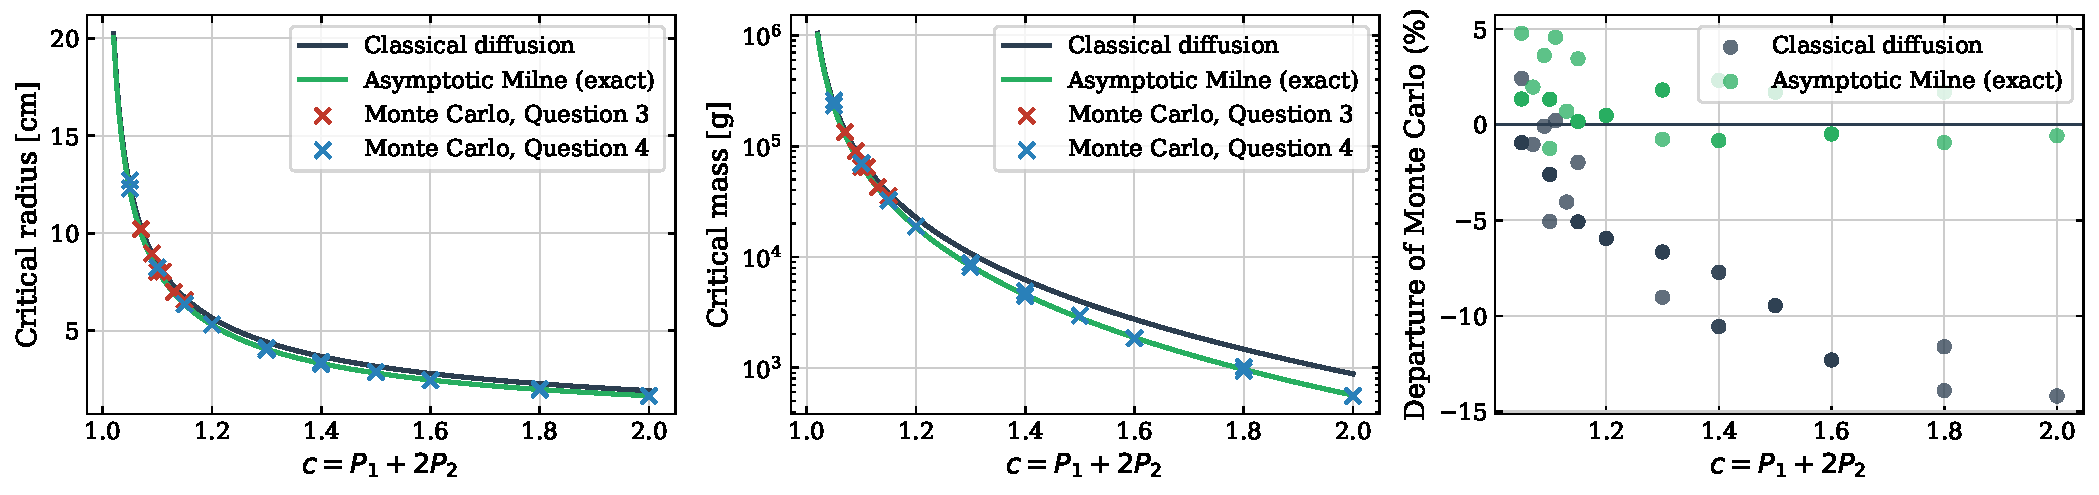
\includegraphics[width=\textwidth]{figs/analytic_comparison.pdf}
    \caption{Critical radius and critical mass against $c$, for the Monte Carlo sweeps of
    Questions 3 and 4 and the two analytical approximations. The right panel is the signed
    departure of each Monte Carlo radius from each theory.}
    \label{fig:analytic}
\end{figure}


\begin{table}[hbt!]
    \centering
    \begin{tabular}{lrrr}
        \toprule
        & & \multicolumn{2}{c}{Departure of Monte Carlo (\%)} \\
        \cmidrule(lr){3-4}
        $c$ & $R_{\text{MC}}$ [cm] & Classical & Asymptotic Milne \\
        \midrule
        1.05 & 12.361 & $-0.38$ & $+1.92$ \\
        1.07 & 10.208 & $-1.03$ & $+1.97$ \\
        1.09 &  8.958 & $-0.08$ & $+3.62$ \\
        1.10 &  8.199 & $-2.95$ & $+0.96$ \\
        1.11 &  8.021 & $+0.22$ & $+4.57$ \\
        1.13 &  6.979 & $-4.04$ & $+0.71$ \\
        1.15 &  6.384 & $-4.64$ & $+0.63$ \\
        1.20 &  5.313 & $-5.95$ & $+0.49$ \\
        1.30 &  4.089 & $-7.25$ & $+1.17$ \\
        1.40 &  3.333 & $-9.14$ & $+0.74$ \\
        1.50 &  2.865 & $-9.46$ & $+1.70$ \\
        1.60 &  2.448 & $-12.31$ & $-0.48$ \\
        1.80 &  1.979 & $-12.76$ & $+0.38$ \\
        2.00 &  1.641 & $-14.19$ & $-0.58$ \\
        \bottomrule
    \end{tabular}
    \caption{Mean Monte Carlo critical radius at each distinct $c$, against the two
    approximations. Configurations sharing a $c$ are averaged.}
    \label{tab:analytic}
\end{table}


\subsection*{Discussion}

The asymptotic Milne curve tracks the Monte Carlo over the whole range, staying inside $\pm 2\%$
except at two low-$c$ points, while the classical curve drifts steadily away, from a fraction of a
per cent near $c = 1$ to $-14\%$ at $c = 2$. The bisection stops at $dr < 0.05r$, so a Monte Carlo
radius is itself only determined to about $\pm 2.5\%$. The asymptotic agreement is therefore at
the noise floor of the simulation, and the point-to-point scatter in the departure panel of
Figure~\ref{fig:analytic} is the stopping rule rather than a failure of the theory.

Classical diffusion is accurate near $c = 1$ because that is the limit in which the $P_1$ closure
it rests on becomes exact. As $c \to 1$ the medium neither absorbs nor multiplies on average, a
Studention survives many collisions before it is lost, and the angular flux relaxes to
near-isotropy between events. Formally, the diffusion relaxation length
and the true one converge in that limit: $1/B$ exceeds $|\nu_0|$ by only $2\%$ at $c = 1.05$,
because both diverge like $[3(c-1)]^{-1/2}$ (actually, this was derived in the course as the asymptotic limit of the exact $|\nu_0|$ at $c\to1$),

The accuracy falls away as $c$ increases for the same reason in reverse. A strongly multiplying
sphere is critical while it is only a couple of mean free paths across so that the leakage is a large fraction of the total loss, and the angular
distribution near the surface is strongly forward-peaked. This is where the $P_1$ closure fails, yet the asymptotic Milne curve remains accurate because it is based on the exact relaxation length.
\end{document}
